
\subsection{Tuning with multiple midpoints}

Here is our example curve, from which we build a grammar with hand-chosen rules.

\includegraphics[width=2in]{./3.em/multi_tuning/examples.eps}

We then enrich the grammar by adding in several copies of each rule,
with jittered midpoints

Here are our training curves:
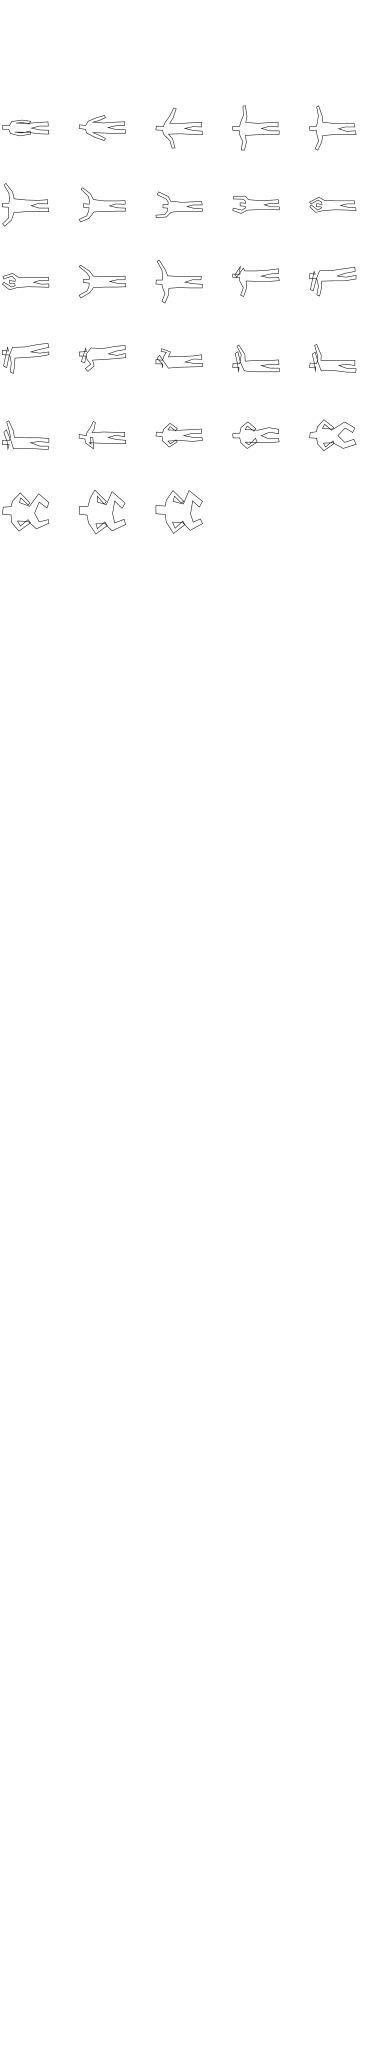
\includegraphics[width=2in]{./3.em/multi_tuning/training.eps}

Here is the grammar:

\subsubsection{Initial}
Here are some samples from the grammar:

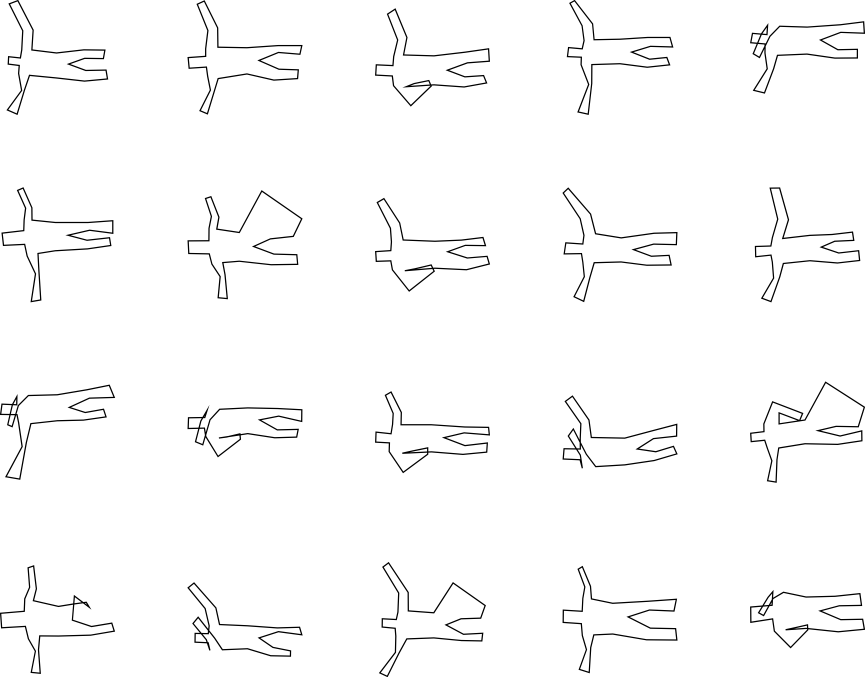
\includegraphics[width=6in]{output/3.learning/incremental/gram.19.d/samples.png}



\subsubsection{Round 1}
Here are some samples from the grammar:

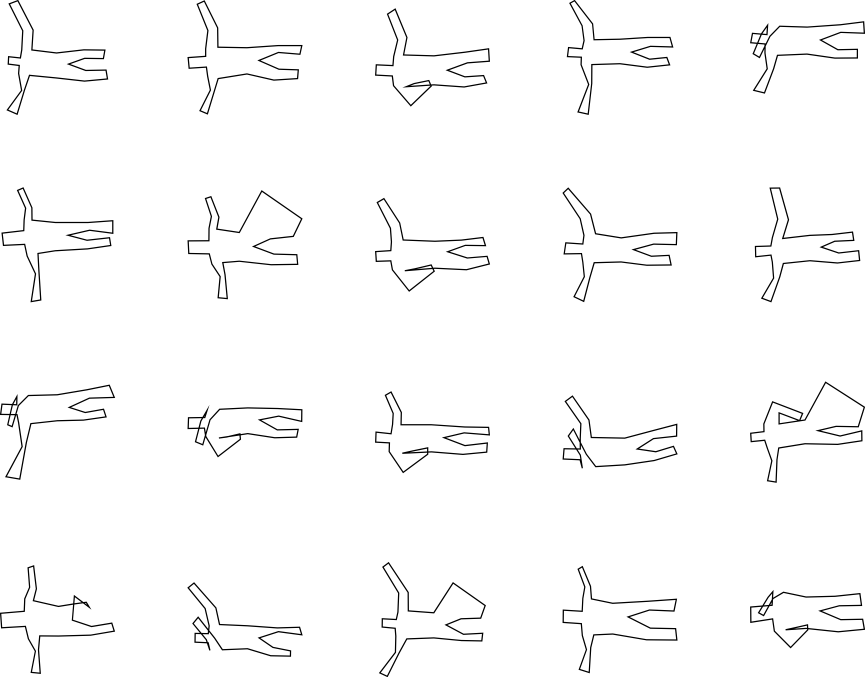
\includegraphics[width=6in]{output/3.learning/incremental/gram.19.d/samples.png}


\subsubsection{Round 2}
Here are some samples from the grammar:

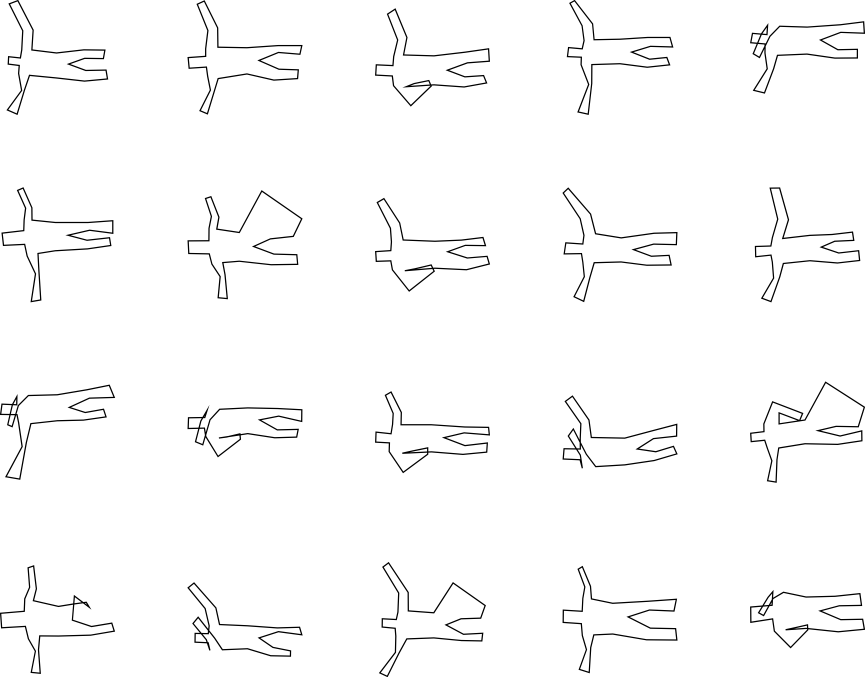
\includegraphics[width=6in]{output/3.learning/incremental/gram.19.d/samples.png}


\subsubsection{Round 3}
Here are some samples from the grammar:

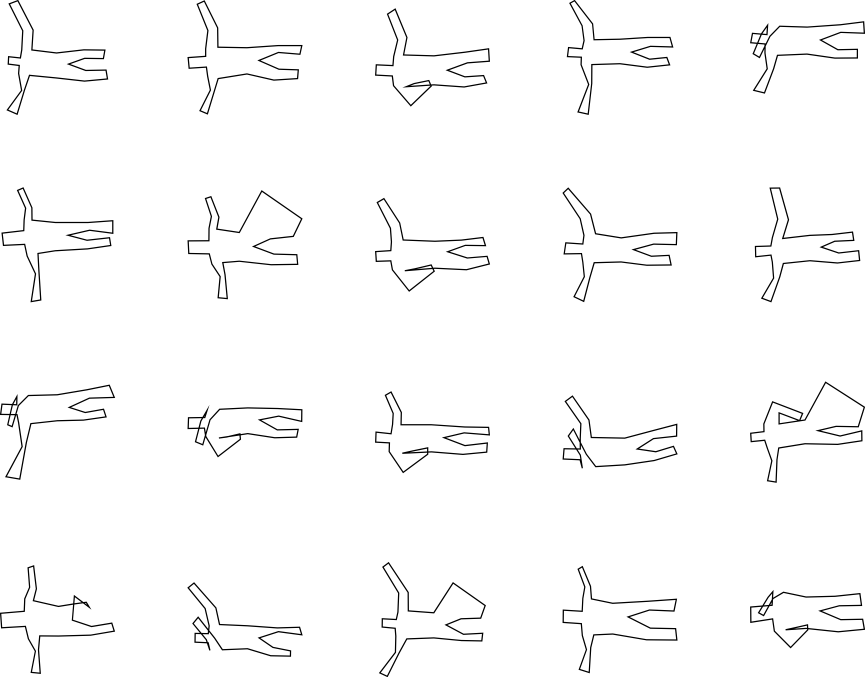
\includegraphics[width=6in]{output/3.learning/incremental/gram.19.d/samples.png}


\subsubsection{Round 4}
Here are some samples from the grammar:

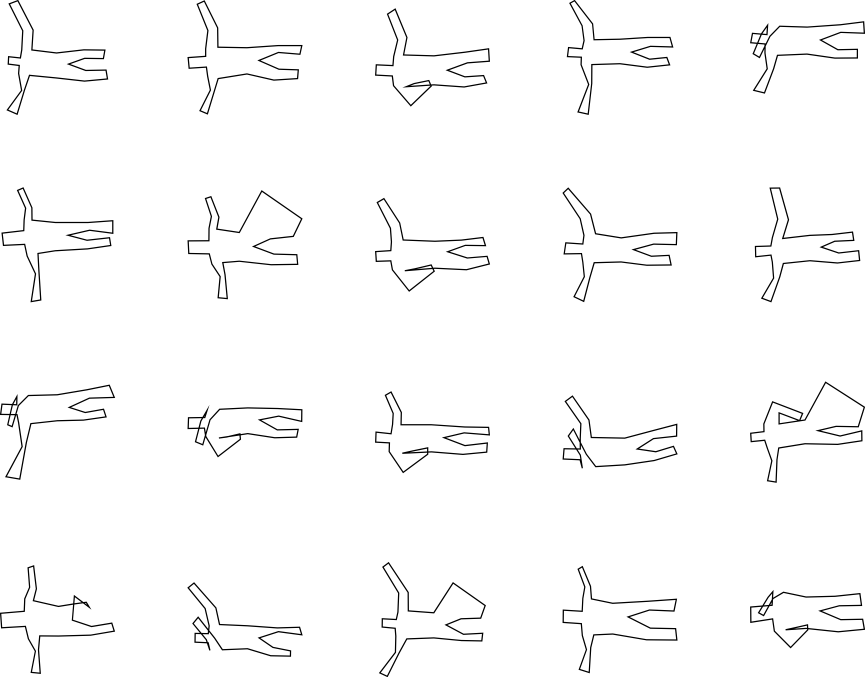
\includegraphics[width=6in]{output/3.learning/incremental/gram.19.d/samples.png}


\subsubsection{Round 5}
Here are some samples from the grammar:

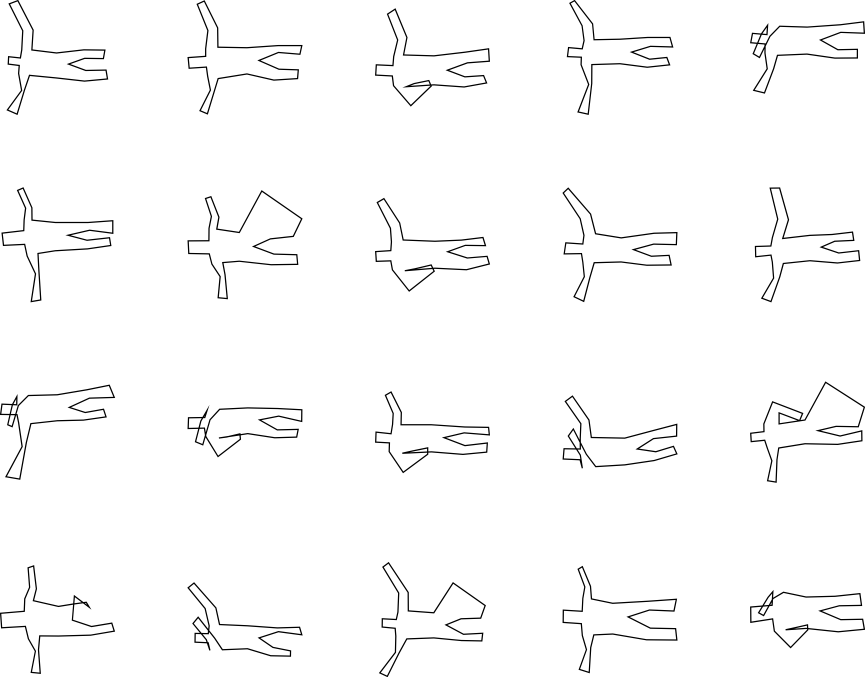
\includegraphics[width=6in]{output/3.learning/incremental/gram.19.d/samples.png}


